\chapter{Introduction to Statistical Sciences}

\section{What is statistics about?}

Stat 230 was about \emph{probability}: given a model, what data should we expect? Stat 231
turns this around. Given \emph{data}, what can we learn about the process or population
that produced it, and how sure can we be? Statistical science is the discipline of
planning studies, collecting data, analysing it with models that account for variability,
and drawing conclusions with an honest statement of uncertainty.

\begin{definition}[Empirical study]
An \emph{empirical study} is one in which knowledge is gained by observation or
experiment, i.e.\ by collecting data, rather than purely by theory.
\end{definition}

Examples: estimating the fraction of Ontario voters who support a party (a \emph{sample
survey}); measuring whether a new fertilizer increases crop yield (an \emph{experimental
study}); studying whether smoking is associated with lung cancer using hospital records
(an \emph{observational study}).

\subsection{Units, populations and processes}

\begin{definition}
\begin{itemize}
  \item A \emph{unit} is an individual person, place or thing about which we take
        measurements.
  \item A \emph{population} is a collection of units (finite and existing, e.g.\ all
        UW undergraduates in Fall 2019).
  \item A \emph{process} is a mechanism that generates units over time (e.g.\ the
        stream of light bulbs produced by a factory, or calls arriving at a call centre).
        Populations of units generated by processes are typically unbounded/conceptual.
\end{itemize}
\end{definition}

\begin{definition}[Variates]
A \emph{variate} is a characteristic of a unit, usually denoted by a letter such as
$x$ or $y$. Types of variates:
\begin{itemize}
  \item \textbf{continuous}: measured on a continuous scale (height, time, weight);
  \item \textbf{discrete}: takes countably many (usually integer) values (number of
        accidents, number of defects);
  \item \textbf{categorical}: unit falls into one of a set of non-numerical categories
        (hair colour, blood type, program of study);
  \item \textbf{ordinal}: categorical with a natural order (strongly disagree,
        disagree, neutral, agree, strongly agree);
  \item \textbf{complex}: images, text, curves, sequences.
\end{itemize}
\end{definition}

\begin{definition}[Attribute]
An \emph{attribute} of a population or process is a function of the variates over the
whole population: e.g.\ the population mean height, the proportion of smokers, the
correlation between two variates. Attributes are usually unknown; the goal of a study is
to learn about them from a sample.
\end{definition}

\begin{remark}
Statistical questions are often classified as \emph{descriptive} (what is the value of
an attribute?), \emph{causative} (does changing $x$ cause a change in $y$?), or
\emph{predictive} (what will $y$ be for a new unit?).
\end{remark}

\section{Numerical data summaries}

Suppose we have data $y_1,\dots,y_n$ on a single variate, with order statistics
$y_{(1)} \le y_{(2)} \le \dots \le y_{(n)}$.

\subsection{Measures of location}

\begin{definition}
\begin{itemize}
  \item \emph{Sample mean}: $\ybar = \dfrac{1}{n}\sum_{i=1}^n y_i$.
  \item \emph{Sample median} $\hat m$: the middle value, $y_{((n+1)/2)}$ if $n$ is odd and
        $\tfrac12\big(y_{(n/2)} + y_{(n/2+1)}\big)$ if $n$ is even.
  \item \emph{Sample mode}: the most frequent value (or the class with the highest
        frequency in a grouped summary).
\end{itemize}
\end{definition}

The median is \emph{robust}: a single huge outlier changes the mean a lot but the median
hardly at all.

\begin{definition}[Sample quantiles]
For $0<p<1$, the $p$th \emph{sample quantile} $q(p)$ is a value such that roughly a
fraction $p$ of the data lie at or below it. One common convention (used in these notes):
let $m = (n+1)p$. If $m$ is an integer, $q(p) = y_{(m)}$; otherwise, with
$k=\floor{m}$, interpolate:
\[
q(p) = y_{(k)} + (m-k)\big(y_{(k+1)} - y_{(k)}\big).
\]
The \emph{lower quartile} is $q(0.25)$, the median is $q(0.5)$ and the \emph{upper
quartile} is $q(0.75)$. Different software packages use slightly different conventions;
for large $n$ they agree closely.
\end{definition}

\subsection{Measures of variability (dispersion)}

\begin{definition}
\begin{itemize}
  \item \emph{Sample variance}: $s^2 = \dfrac{1}{n-1}\sum_{i=1}^n (y_i-\ybar)^2
        = \dfrac{1}{n-1}\Big(\sum y_i^2 - n\ybar^2\Big)$, and \emph{sample standard
        deviation} $s=\sqrt{s^2}$.
  \item \emph{Range}: $y_{(n)} - y_{(1)}$.
  \item \emph{Interquartile range}: $\mathrm{IQR} = q(0.75) - q(0.25)$.
\end{itemize}
\end{definition}

The divisor $n-1$ (rather than $n$) makes $S^2$ an unbiased estimator of $\sigma^2$
(see Chapter 4). The IQR, like the median, is robust to outliers.

\subsection{Measures of shape}

\begin{definition}
\begin{itemize}
  \item \emph{Sample skewness}:
  $\displaystyle g_1 = \frac{\frac1n\sum (y_i-\ybar)^3}{\big[\frac1n\sum (y_i-\ybar)^2\big]^{3/2}}$.
  Positive skewness means a long right tail; negative means a long left tail; $g_1\approx
  0$ for symmetric data.
  \item \emph{Sample kurtosis}:
  $\displaystyle g_2 = \frac{\frac1n\sum (y_i-\ybar)^4}{\big[\frac1n\sum (y_i-\ybar)^2\big]^{2}}$.
  For Gaussian data $g_2 \approx 3$; $g_2>3$ indicates heavier tails (more extreme
  values) than the Gaussian, $g_2<3$ lighter tails (e.g.\ uniform data has kurtosis
  $1.8$).
\end{itemize}
\end{definition}


\begin{center}
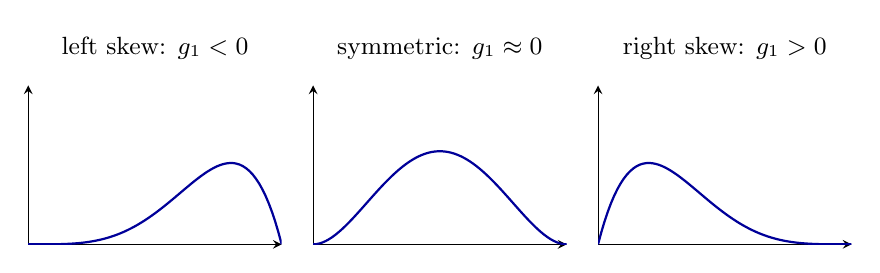
\begin{tikzpicture}
\begin{axis}[name=k1, width=4.8cm, height=3.6cm, xmin=0, xmax=1, ymin=0, ymax=3.2, axis lines=left,
    xtick=\empty, ytick=\empty, title={left skew: $g_1<0$}, title style={font=\small}, samples=80]
  \addplot[thick, blue!60!black, domain=0:1] {20*x^4*(1-x)};
\end{axis}
\begin{axis}[name=k2, at={(k1.east)}, anchor=west, xshift=0.4cm, width=4.8cm, height=3.6cm, xmin=0,
    xmax=1, ymin=0, ymax=3.2, axis lines=left, xtick=\empty, ytick=\empty, title={symmetric: $g_1\approx0$},
    title style={font=\small}, samples=80]
  \addplot[thick, blue!60!black, domain=0:1] {30*x^2*(1-x)^2};
\end{axis}
\begin{axis}[at={(k2.east)}, anchor=west, xshift=0.4cm, width=4.8cm, height=3.6cm, xmin=0, xmax=1,
    ymin=0, ymax=3.2, axis lines=left, xtick=\empty, ytick=\empty, title={right skew: $g_1>0$},
    title style={font=\small}, samples=80]
  \addplot[thick, blue!60!black, domain=0:1] {20*x*(1-x)^4};
\end{axis}
\end{tikzpicture}
\end{center}

\subsection{Bivariate summaries}

For paired data $(x_i,y_i)$, the \emph{sample correlation} is
\[
r = \frac{S_{xy}}{\sqrt{S_{xx}S_{yy}}},\quad
S_{xx}=\sum(x_i-\bar x)^2,\ S_{yy}=\sum(y_i-\ybar)^2,\ S_{xy}=\sum (x_i-\bar x)(y_i-\ybar).
\]
Always $-1\le r\le 1$; $r$ measures the strength of \emph{linear} association only. For two
categorical variates, a \emph{two-way (contingency) table} of counts is the natural summary
(Chapter 7).

\begin{example}[Complete set of numerical summaries]
\label{ex:summ}
The waiting times (minutes) of $n=12$ customers are
\[
3.2,\ 4.1,\ 4.5,\ 5.0,\ 5.3,\ 5.8,\ 6.1,\ 6.4,\ 7.0,\ 7.9,\ 9.6,\ 12.3
\]
(already sorted). Then $\sum y_i = 77.2$, $\sum y_i^2 = 567.06$, so
\[
\ybar = \frac{77.2}{12} = 6.4333,\qquad
S_{yy} = 567.06 - \frac{77.2^2}{12} = 567.06 - 496.6533 = 70.4067,
\]
\[
s^2 = \frac{70.4067}{11} = 6.4006,\qquad s = 2.5299.
\]
\textbf{Quantiles.} For $p=0.25$: $m = 13(0.25) = 3.25$, so
$q(0.25) = y_{(3)} + 0.25(y_{(4)}-y_{(3)}) = 4.5 + 0.25(0.5) = 4.625$.
For $p=0.5$: $m=6.5$, so $\hat m = (5.8+6.1)/2 = 5.95$.
For $p=0.75$: $m = 9.75$, so $q(0.75) = 7.0 + 0.75(0.9) = 7.675$.
Hence $\mathrm{IQR} = 7.675 - 4.625 = 3.05$, and the range is $12.3 - 3.2 = 9.1$.

\textbf{Shape.} With $m_k = \frac1n\sum (y_i-\ybar)^k$ we get $m_2 = 5.8672$,
$m_3 = 14.882$, $m_4 = 120.74$, so
\[
g_1 = \frac{14.882}{5.8672^{3/2}} = 1.047, \qquad g_2 = \frac{120.74}{5.8672^2} = 3.51.
\]
The data are right-skewed (mean $6.43 >$ median $5.95$, $g_1>0$) with slightly heavier
tails than a Gaussian. This is typical of waiting times.
\end{example}

\section{Graphical data summaries}

\subsection{Histograms}
Partition the range into intervals (bins) $[a_0,a_1),[a_1,a_2),\dots,[a_{k-1},a_k)$
and count the frequency $f_j$ in each. A \emph{relative frequency histogram} draws a
rectangle over bin $j$ with \emph{area} $f_j/n$, i.e.\ height $f_j/\big(n(a_j-a_{j-1})\big)$.
Then the total area is $1$ and the histogram can be compared directly with a probability
density function. With unequal bin widths, using heights $=$ frequencies is a classic
mistake: wide bins look too important.

\begin{center}
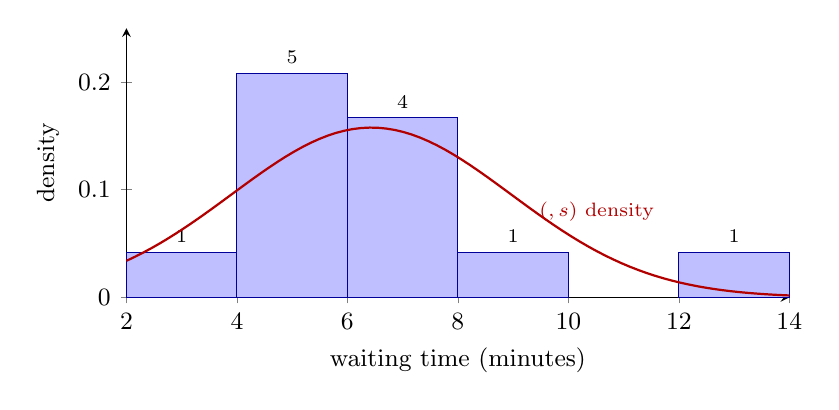
\begin{tikzpicture}
\begin{axis}[width=10cm, height=5cm, xmin=2, xmax=14, ymin=0, ymax=0.25, xtick={2,4,...,14},
    xlabel={waiting time (minutes)}, ylabel={density}, tick label style={font=\small}, label style={font=\small}, axis lines=left, scaled y ticks=false, yticklabel style={/pgf/number format/fixed}, clip=false]
  \draw[fill=blue!25, draw=blue!60!black] (axis cs:2,0) rectangle (axis cs:4,0.0417);
  \node[font=\scriptsize, above] at (axis cs:3.0,0.0417) {1};
  \draw[fill=blue!25, draw=blue!60!black] (axis cs:4,0) rectangle (axis cs:6,0.2083);
  \node[font=\scriptsize, above] at (axis cs:5.0,0.2083) {5};
  \draw[fill=blue!25, draw=blue!60!black] (axis cs:6,0) rectangle (axis cs:8,0.1667);
  \node[font=\scriptsize, above] at (axis cs:7.0,0.1667) {4};
  \draw[fill=blue!25, draw=blue!60!black] (axis cs:8,0) rectangle (axis cs:10,0.0417);
  \node[font=\scriptsize, above] at (axis cs:9.0,0.0417) {1};
  \draw[fill=blue!25, draw=blue!60!black] (axis cs:12,0) rectangle (axis cs:14,0.0417);
  \node[font=\scriptsize, above] at (axis cs:13.0,0.0417) {1};
  \addplot[thick, red!70!black, domain=2:14, samples=80] {exp(-(x-6.4333)^2/(2*6.4006))/sqrt(2*pi*6.4006)};
  \node[font=\scriptsize, text=red!70!black, anchor=west] at (axis cs:9.3,0.08) {$\Gau(\ybar, s)$ density};
\end{axis}
\end{tikzpicture}
\end{center}
A relative frequency histogram of the waiting times of Example~\ref{ex:summ} (bins of width
$2$; counts above the bars). Because the bar areas sum to $1$, a fitted Gaussian density can
be drawn on the same scale; the long right tail does not match it well.

\subsection{Empirical cumulative distribution function}

\begin{definition}[ECDF]
$\hat F(y) = \dfrac{\#\{i : y_i \le y\}}{n}$, a step function jumping by $1/n$ at each
observation. It estimates the population c.d.f.\ $F(y) = \Prob(Y\le y)$.
\end{definition}

The ECDF uses all the data (no binning choice) and quantiles can be read off it. To check
a model, plot $\hat F$ together with the fitted model c.d.f.

\begin{center}
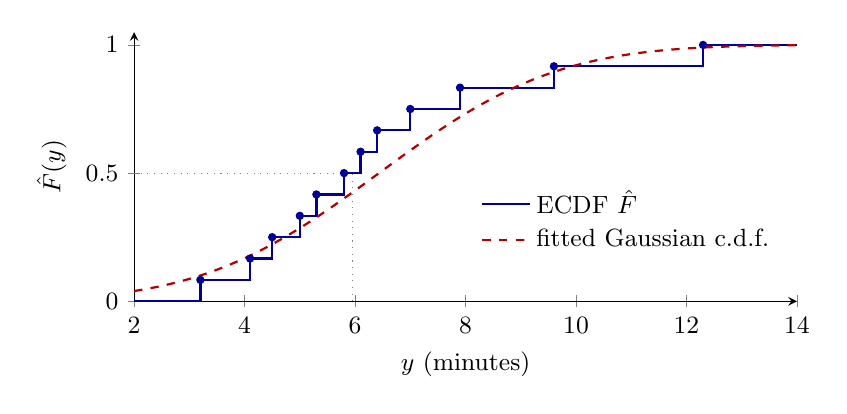
\begin{tikzpicture}
\begin{axis}[width=10cm, height=5cm, xmin=2, xmax=14, ymin=0, ymax=1.05, xtick={2,4,...,14},
    xlabel={$y$ (minutes)}, ylabel={$\hat F(y)$}, tick label style={font=\small}, label style={font=\small}, axis lines=left, scaled y ticks=false, yticklabel style={/pgf/number format/fixed}, legend style={font=\small, draw=none,
    at={(0.98,0.3)}, anchor=east}, legend cell align=left]
  \addplot[const plot, thick, blue!60!black] coordinates {(2,0) (3.2,0.0833) (4.1,0.1667) (4.5,0.2500) (5.0,0.3333) (5.3,0.4167) (5.8,0.5000) (6.1,0.5833) (6.4,0.6667) (7.0,0.7500) (7.9,0.8333) (9.6,0.9167) (12.3,1.0000) (14,1)};
  \addplot[thick, red!70!black, dashed, smooth] coordinates {(2.00,0.0399) (2.25,0.0491) (2.50,0.0600) (2.75,0.0727) (3.00,0.0874) (3.25,0.1041) (3.50,0.1231) (3.75,0.1444) (4.00,0.1681) (4.25,0.1941) (4.50,0.2224) (4.75,0.2529) (5.00,0.2855) (5.25,0.3200) (5.50,0.3561) (5.75,0.3935) (6.00,0.4320) (6.25,0.4711) (6.50,0.5105) (6.75,0.5498) (7.00,0.5886) (7.25,0.6266) (7.50,0.6634) (7.75,0.6986) (8.00,0.7321) (8.25,0.7636) (8.50,0.7930) (8.75,0.8201) (9.00,0.8448) (9.25,0.8672) (9.50,0.8873) (9.75,0.9051) (10.00,0.9207) (10.25,0.9343) (10.50,0.9460) (10.75,0.9560) (11.00,0.9645) (11.25,0.9715) (11.50,0.9774) (11.75,0.9822) (12.00,0.9861) (12.25,0.9893) (12.50,0.9918) (12.75,0.9937) (13.00,0.9953) (13.25,0.9965) (13.50,0.9974) (13.75,0.9981) (14.00,0.9986)};
  \addplot[only marks, mark=*, mark size=1.3pt, blue!60!black, forget plot] coordinates {(3.2,0.0833) (4.1,0.1667) (4.5,0.2500) (5.0,0.3333) (5.3,0.4167) (5.8,0.5000) (6.1,0.5833) (6.4,0.6667) (7.0,0.7500) (7.9,0.8333) (9.6,0.9167) (12.3,1.0000)};
  \draw[gray, dotted] (axis cs:2,0.5) -- (axis cs:5.95,0.5) -- (axis cs:5.95,0);
  \legend{ECDF $\hat F$, {fitted Gaussian c.d.f.}}
\end{axis}
\end{tikzpicture}
\end{center}
The ECDF of the waiting times jumps by $1/12$ at each observation; reading across at
height $0.5$ gives the median (dotted). The dashed curve is the Gaussian c.d.f.\ with the
sample mean and standard deviation.

\subsection{Boxplots}
A \emph{boxplot} draws a box from $q(0.25)$ to $q(0.75)$ with a line at the median.
Whiskers extend to the most extreme observations within $1.5\,\mathrm{IQR}$ of the box;
points beyond that are plotted individually as possible outliers. Side-by-side boxplots
are excellent for comparing groups.

\begin{example}[Boxplot of the waiting times]
In Example~\ref{ex:summ}, $1.5\,\mathrm{IQR} = 4.575$, so the fences are
$4.625 - 4.575 = 0.05$ and $7.675 + 4.575 = 12.25$. The value $12.3$ exceeds the upper
fence, so it is plotted as an outlier and the upper whisker stops at $9.6$; the lower
whisker goes to $3.2$.
\begin{center}
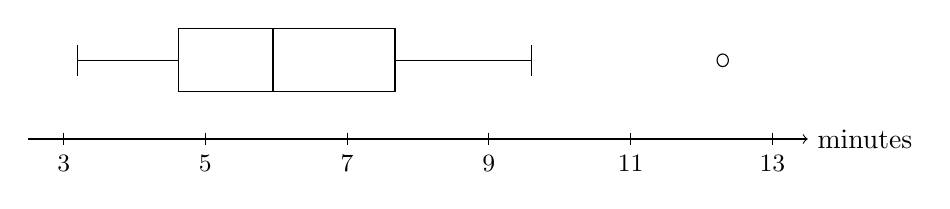
\begin{tikzpicture}[x=0.9cm,y=1cm]
  \draw[->] (2.5,0) -- (13.5,0) node[right] {minutes};
  \foreach \t in {3,5,7,9,11,13} \draw (\t,0.08) -- (\t,-0.08) node[below] {\small \t};
  \draw (4.625,0.6) rectangle (7.675,1.4);
  \draw[thick] (5.95,0.6) -- (5.95,1.4);
  \draw (3.2,1) -- (4.625,1); \draw (7.675,1) -- (9.6,1);
  \draw (3.2,0.8) -- (3.2,1.2); \draw (9.6,0.8) -- (9.6,1.2);
  \draw (12.3,1) circle (0.08);
\end{tikzpicture}
\end{center}
The longer right whisker and the outlier both display the right skewness.
\end{example}

\subsection{Scatterplots and run charts}
For bivariate data $(x_i,y_i)$ a \emph{scatterplot} shows the form (linear, curved),
direction and strength of a relationship and reveals outliers. A \emph{run chart} plots a
variate against time order to show trends or shifts in a process.

\subsection{Gaussian QQ plots}

\begin{definition}[QQ plot]
To check whether data look like a sample from a Gaussian distribution, plot the ordered
data $y_{(i)}$ against the theoretical standard normal quantiles $z_i$ with
$\Phi(z_i) = \frac{i}{n+1}$ (or a similar plotting position). If the data are Gaussian,
$y_{(i)} \approx \mu + \sigma z_i$, so the points should lie close to a straight line.
\end{definition}

How to read a QQ plot:
\begin{itemize}
  \item points on a straight line: Gaussian model reasonable (slope $\approx\sigma$,
        intercept $\approx\mu$);
  \item concave-up (``U'') shape: right skew; concave-down: left skew;
  \item an ``S'' shape with both ends pulled away from the line: tails heavier than
        Gaussian (kurtosis $>3$); the reverse S: lighter tails;
  \item some wiggle at the very ends is normal for small $n$, so don't over-interpret.
\end{itemize}

\begin{center}
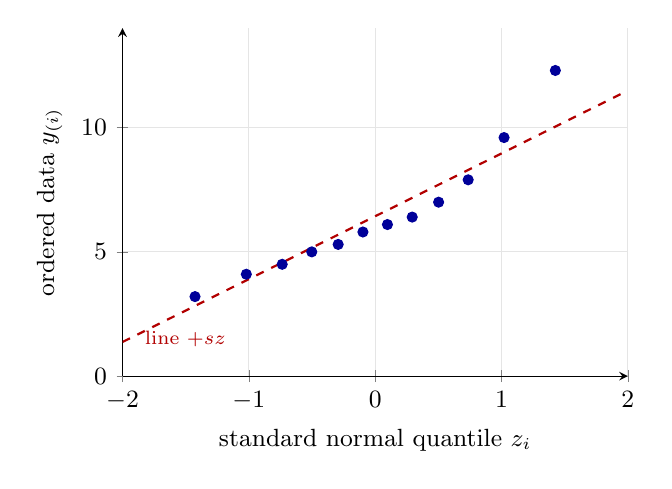
\begin{tikzpicture}
\begin{axis}[width=8cm, height=6cm, xmin=-2, xmax=2, ymin=0, ymax=14, xlabel={standard normal quantile $z_i$},
    ylabel={ordered data $y_{(i)}$}, tick label style={font=\small}, label style={font=\small}, axis lines=left, scaled y ticks=false, yticklabel style={/pgf/number format/fixed}, grid=major, grid style={gray!20}]
  \addplot[thick, red!70!black, dashed, domain=-2:2] {6.4333+2.5299*x};
  \addplot[only marks, mark=*, mark size=1.8pt, blue!60!black] coordinates {(-1.426,3.2) (-1.020,4.1) (-0.736,4.5) (-0.502,5.0) (-0.293,5.3) (-0.097,5.8) (0.097,6.1) (0.293,6.4) (0.502,7.0) (0.736,7.9) (1.020,9.6) (1.426,12.3)};
  \node[font=\scriptsize, text=red!70!black, anchor=west] at (axis cs:-1.9,1.5) {line $\ybar + s z$};
\end{axis}
\end{tikzpicture}
\end{center}
For the $12$ waiting times, the points bend upward at the right end (the largest values are
too large for a Gaussian): the concave-up pattern of right skewness.

\begin{important}[Common pitfalls]
\begin{itemize}
  \item The sample variance divides by $n-1$, not $n$.
  \item Correlation measures \emph{linear} association: $r\approx 0$ does not mean ``no
        relationship'' (e.g.\ $y=x^2$ on symmetric $x$), and large $|r|$ does not imply
        causation (Chapter 8).
  \item Histogram areas, not heights, represent relative frequency.
  \item Always plot the data before computing summaries: means and standard deviations
        can hide outliers, skewness and multiple modes.
\end{itemize}
\end{important}

\section*{Summary}
\begin{itemize}
  \item Empirical studies collect data on \emph{units} from a \emph{population} or
        \emph{process}; we measure \emph{variates} and want to learn about
        \emph{attributes}.
  \item Location: mean, median, mode. Spread: variance/standard deviation, range, IQR.
        Shape: skewness ($0$ for symmetric) and kurtosis ($3$ for Gaussian).
  \item Graphs: histograms (area $=$ relative frequency), ECDF, boxplots
        ($1.5\,\mathrm{IQR}$ rule), scatterplots, and Gaussian QQ plots (straight line
        means Gaussian).
\end{itemize}
